\documentclass{article}

\usepackage[margin=1in]{geometry}
\usepackage{syntax}
\usepackage{float}
\usepackage{amsmath}
\usepackage{tikz}
\usetikzlibrary{arrows,automata}
\usepackage{minted}

\title{Deep Strictness: Milestone 1}
\author{Kenny, Hengchu}

\begin{document}
\maketitle

At the first phase of the project, we have investigated the objects in
our abstract domain for characterizing strictness of a subset of GHC
Core.

In particular, we have restricted our scope to functions that take a
single argument, and produces a single argument. However, we place no
constraint on the types of the input and output. They can be terms of
arbitrary user-defined algebraic data types as input.

An example of such a function is \verb|half|, which divides a natural
number by $2$.

\begin{minted}{haskell}
-- |The data type of natural numbers
data Nat = Z     -- ^ Zero
         | S Nat -- ^ Successor of a natural number

half :: Nat -> Nat
half n =
  case! n of
    Z    -> Z
    S n' -> case! n' of
              Z     -> Z
              S n'' -> S (half n'')
\end{minted}

The \verb|half| function pattern matches on the input number, and
returns $0$ if the input is either $0$ or $1$, and if the input is $2$
successor constructors applied to some other natural number, then it
recursively invokes itself on that natural number, and finally applies
a constructor to the result of the recursive computation. We will use
\verb|half| as the running example in the following discussion.

Our first observation is that we can use a graph to represent the
structure of an algebraic data type, with the internal nodes
correspond to choices of constructors and projection of arguments
applied to constructors. Concretely, the \verb|Nat| type is
represented by this graph:

\begin{figure}[H]
  \centering
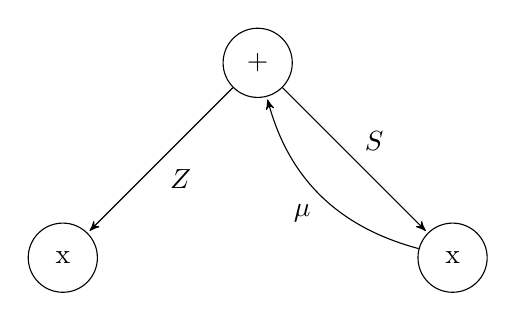
\begin{tikzpicture}[->,>=stealth',shorten >=1pt,auto,node distance=3.5cm,
        scale = 1,transform shape]

  \node[state] (top)                        {+};
  \node[state] (left)  [below left of=top]  {x};
  \node[state] (right) [below right of=top] {x};

  \path (top)   edge              node {$Z$} (left)
        (top)   edge              node {$S$} (right)
        (right) edge [bend left]  node {$\mu$} (top);

\end{tikzpicture}
\end{figure}

The \verb|+| node represents the choice between constructor \verb|Z|
and constructor \verb|S| in a natural number, where the $\mu$ edge
represents the recursive structure of \verb|Nat| --- the field of the
successor constructor is also a natural number.

Having the type of \verb|Nat| represented as a graph is a first step
towards exploring representations of strictness in this format. We
also need a control flow graph of the function under the analysis. In
this case, the half function can be represented by the following CFG:

\begin{figure}[H]
  \centering
\begin{tikzpicture}[->,>=stealth',shorten >=1pt,auto,node distance=3.5cm,
        scale = 1,transform shape]

  \node[state] (n)  {\verb|n|};
  \node[state] (z0) [below left of=n] {\verb|Z|};
  \node[state] (s0) [below right of=n] {\verb|n'|};
  \node[state] (z1) [below left of=s0] {\verb|Z|};
  \node[state] (s1) [below right of=s0] {\verb|n''|};

  \path (n) edge               node {$$} (z0)
        (n) edge               node {$$} (s0)
        (s0) edge              node {$$} (z1)
        (s0) edge              node {$$} (s1)
        (s1) edge [bend right] node {$$} (n);
\end{tikzpicture}
\end{figure}

The CFG can be interpreted as the following: the function \verb|half|
branches on the variable $n$, and returns if $n$ is \verb|Z|, or it
branches on the predecessor $n'$ of $n$, and terminates if $n'$ is
\verb|Z|, otherwise it recurses on the predecessor $n''$ of $n'$.

Now, we can connect the nodes on the type \verb|Nat| and the nodes on
the CFG of \verb|half| to approximate the strictness behavior.

\begin{figure}[H]
  \centering
  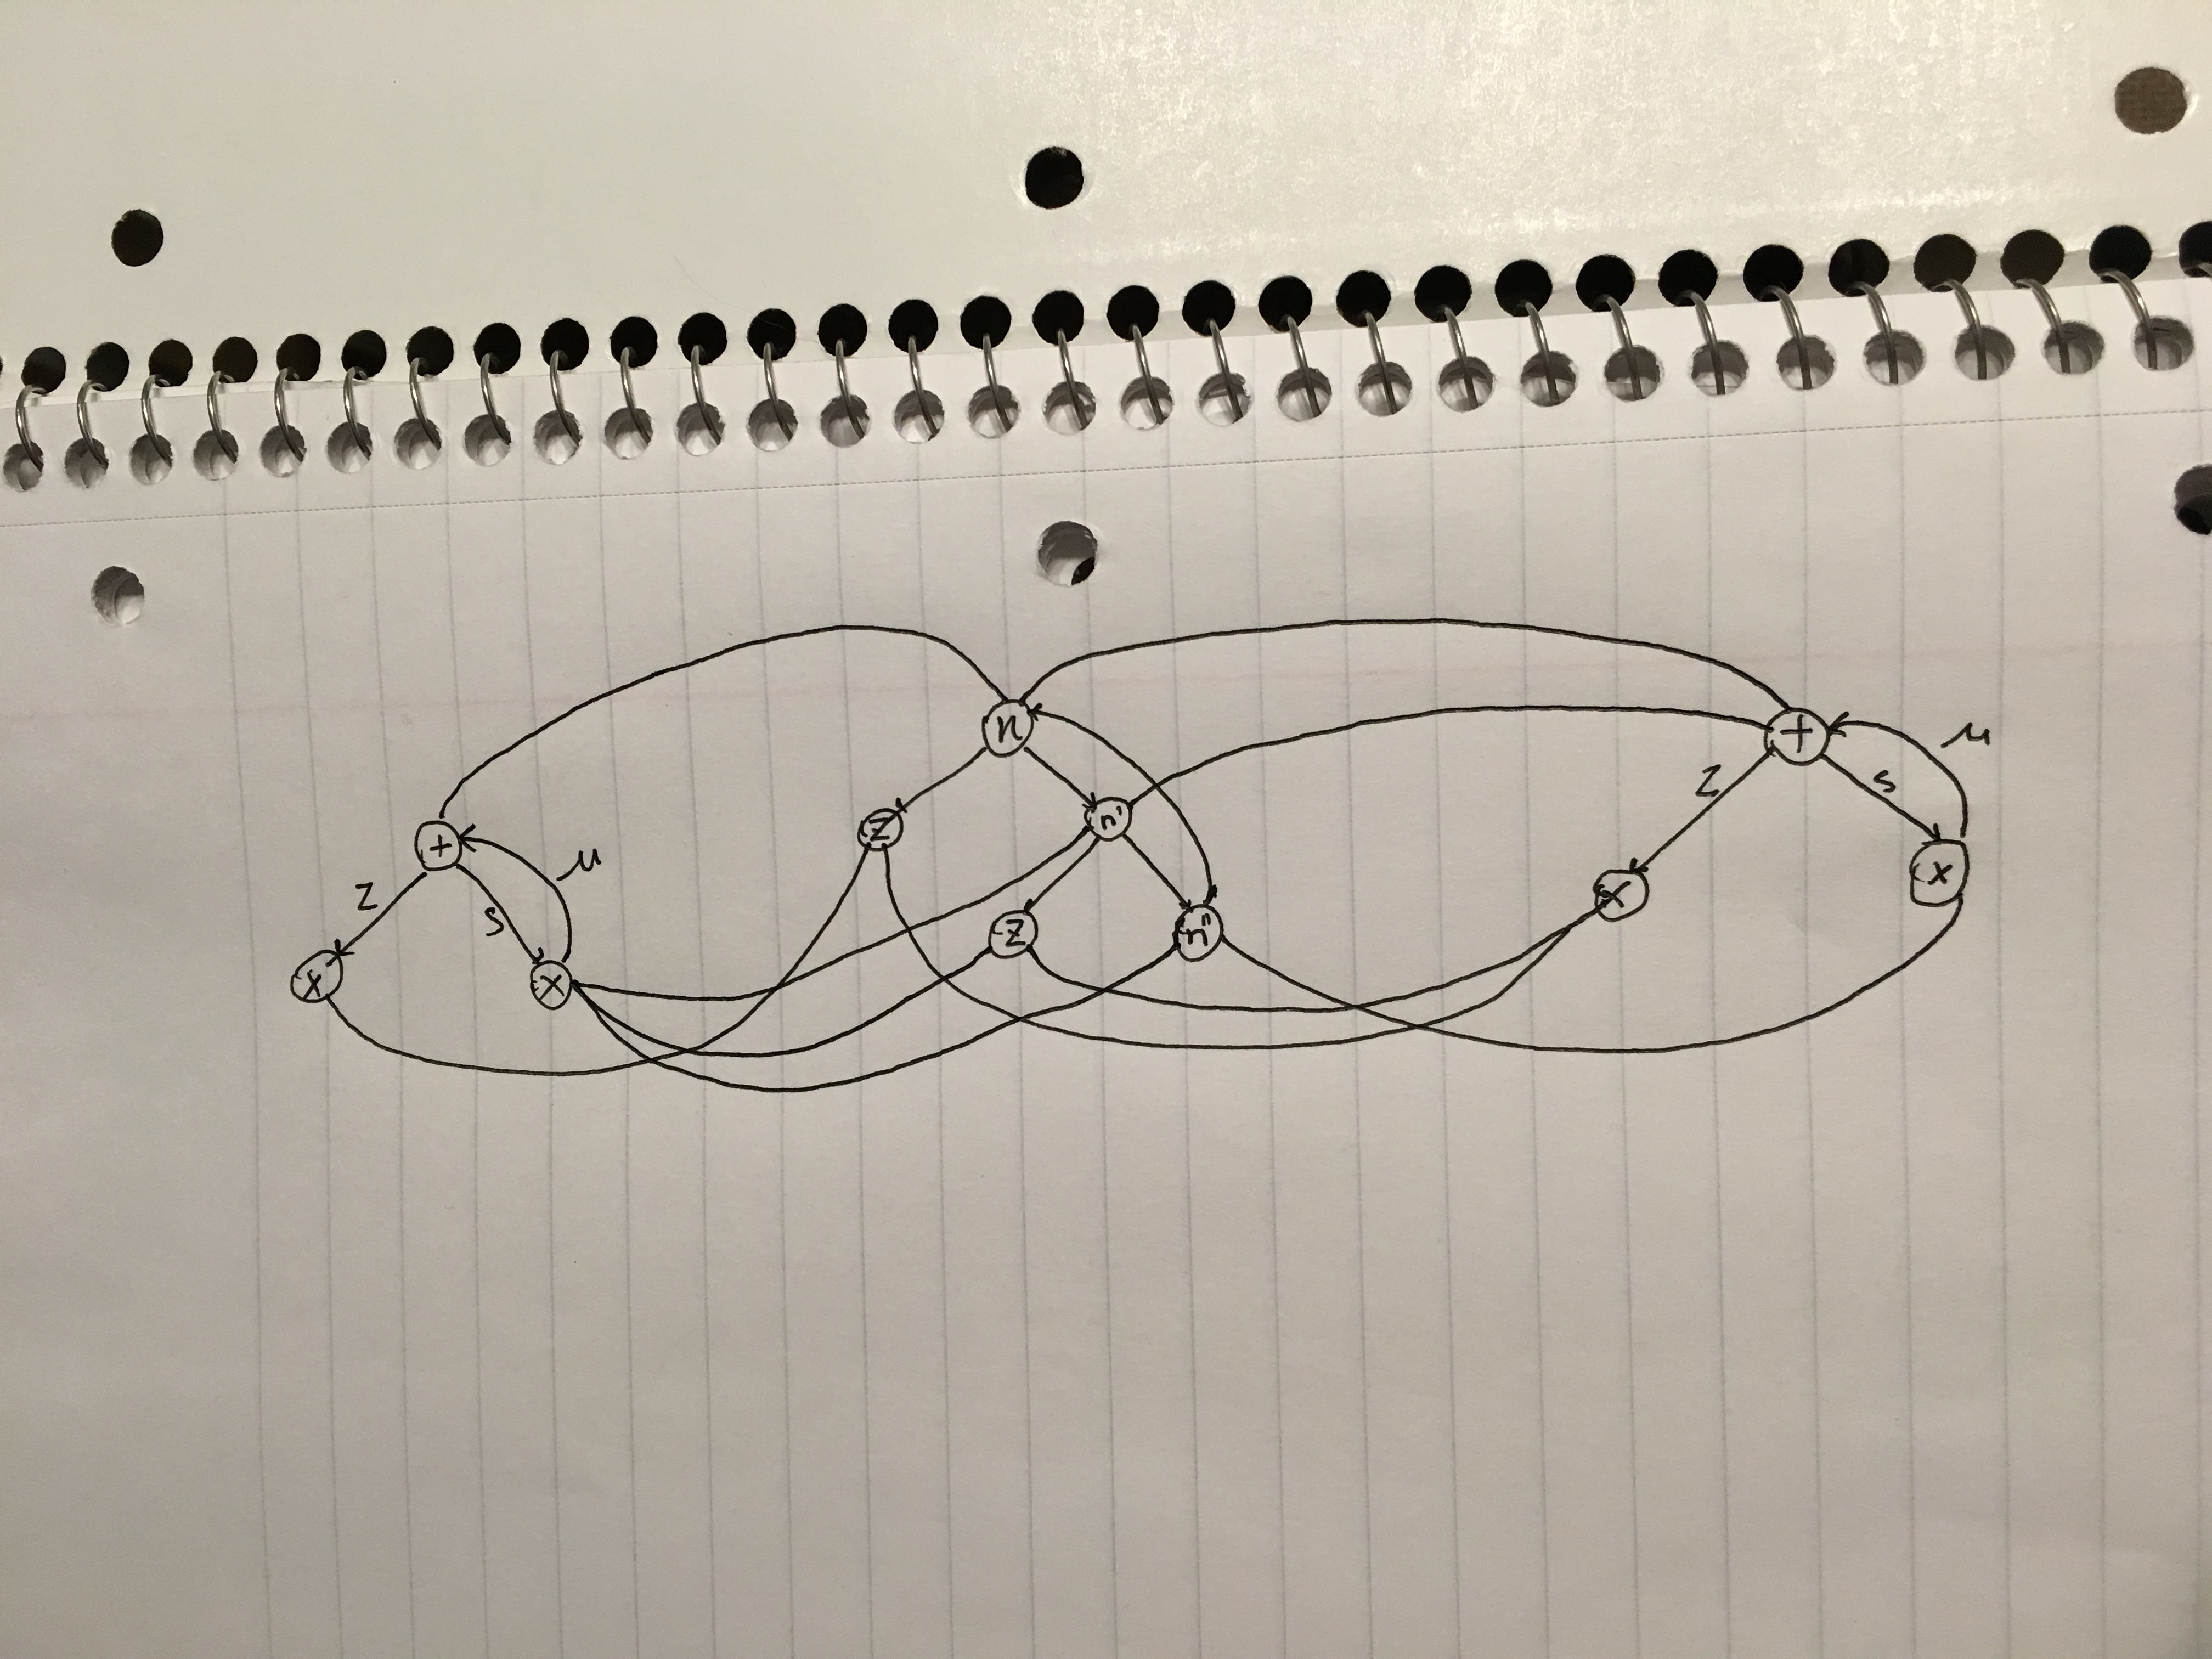
\includegraphics[width=0.7\textwidth]{half}
  \caption{Strictness graph of \texttt{half}}
\end{figure}

Here, the graph on the righthand side propagates demand of the output
through the control flow graph, back to the input on the lefthand
side. The way to read this graph is

\begin{enumerate}
  \item \verb|half| produces nothing at nodes $n$ and $n'$. Hence,
    they're connected to the top node on the RHS, which has not
    produced any constructors yet.

  \item \verb|half| produces a \verb|Z| constructor when $n$ turns out
    to be zero. Hence, it is connected to the \verb|x| node following
    the \verb|Z| branch on the RHS.

  \item \verb|half| also produces \verb|Z| when $n'$ turns out to be
    zero. Hence the connection between the lower \verb|Z| node and the
    left \verb|x| node following the \verb|Z| branch on the RHS.

  \item \verb|half| produces a \verb|S| constructor when $n'$ turns
    out to be the successor of some number $n''$. Hence, there is a
    connection between $n''$ and the \verb|x| node following the
    \verb|S| branch.

  \item We also connect all the pattern matching points to where the
    sums occur on the LHS. Since we pattern match on $n$, which
    corresponds to the top level \verb|+| node on the LHS, there is an
    edge between them. Similarly, there is an edge between \verb|x|
    following the \verb|S| branch to the node $n'$. Note that the same
    \verb|x| is also connected to $n''$, here is where we lose some
    precision on exactly where $n''$ occurs in the structure of the
    input. However, the precision can be improved by unrolling the
    LHS's recursion a few times.
\end{enumerate}

The graph of \verb|half| captures a sound approximation of the
function's strictness behavior. We conjecture that there is in fact a
class of functions whose strictness behavior can be soundly
approximated like this.

Also, conceptually, the graph above describes a Finite State
Transducer, which is a variant of Non-deterministic Finite State
Automata that has an input tape and an output tape, and the transition
graph has the same restrictions as an NFA. In this case, the input
tape holds the constructors that one demands of the output, and the
output tape outputs the constructors one \textit{may} have forced on
the input. This seems to suggest some form of regularness of the
functions that can be characterized by such graphs.

One example that cannot be represented by graphs like this is a
degenerate \verb|swap| function that infinitely changes the position
of its two arguments.

\begin{minted}{haskell}
badSwap :: (a, a) -> a
badSwap p =
  case! p of
    (x, y) -> let p' = (y, x) in
              badSwap p'
\end{minted}

The graph is not capable of capturing the change of position of the
first and second elements in the tuple in a sound way, and we're
currently considering solutions to this problem. One could potentially
unroll the recursion in \verb|badSwap| until the order of arguments is
restored, but such methods can quickly break down in situations where
the number of unrolling required is not known statically. Another
solution is to develop a method of distinguishing such ``misbehaving''
functions from the functions whose strictness behavior can be captured
by a graph, and our analysis will simply refuse to give a graph for
these functions.

\end{document}
